% Options for packages loaded elsewhere
\PassOptionsToPackage{unicode}{hyperref}
\PassOptionsToPackage{hyphens}{url}
\PassOptionsToPackage{dvipsnames,svgnames,x11names}{xcolor}
%
\documentclass[
  11pt,
]{article}
\usepackage{amsmath,amssymb}
\usepackage[]{mathpazo}
\usepackage{iftex}
\ifPDFTeX
  \usepackage[T1]{fontenc}
  \usepackage[utf8]{inputenc}
  \usepackage{textcomp} % provide euro and other symbols
\else % if luatex or xetex
  \usepackage{unicode-math}
  \defaultfontfeatures{Scale=MatchLowercase}
  \defaultfontfeatures[\rmfamily]{Ligatures=TeX,Scale=1}
\fi
% Use upquote if available, for straight quotes in verbatim environments
\IfFileExists{upquote.sty}{\usepackage{upquote}}{}
\IfFileExists{microtype.sty}{% use microtype if available
  \usepackage[]{microtype}
  \UseMicrotypeSet[protrusion]{basicmath} % disable protrusion for tt fonts
}{}
\makeatletter
\@ifundefined{KOMAClassName}{% if non-KOMA class
  \IfFileExists{parskip.sty}{%
    \usepackage{parskip}
  }{% else
    \setlength{\parindent}{0pt}
    \setlength{\parskip}{6pt plus 2pt minus 1pt}}
}{% if KOMA class
  \KOMAoptions{parskip=half}}
\makeatother
\usepackage{xcolor}
\usepackage[margin=1in]{geometry}
\usepackage{graphicx}
\makeatletter
\def\maxwidth{\ifdim\Gin@nat@width>\linewidth\linewidth\else\Gin@nat@width\fi}
\def\maxheight{\ifdim\Gin@nat@height>\textheight\textheight\else\Gin@nat@height\fi}
\makeatother
% Scale images if necessary, so that they will not overflow the page
% margins by default, and it is still possible to overwrite the defaults
% using explicit options in \includegraphics[width, height, ...]{}
\setkeys{Gin}{width=\maxwidth,height=\maxheight,keepaspectratio}
% Set default figure placement to htbp
\makeatletter
\def\fps@figure{htbp}
\makeatother
\setlength{\emergencystretch}{3em} % prevent overfull lines
\providecommand{\tightlist}{%
  \setlength{\itemsep}{0pt}\setlength{\parskip}{0pt}}
\setcounter{secnumdepth}{5}
\usepackage{hyperref}
\usepackage{placeins}
\usepackage{booktabs}
\usepackage{longtable}
\usepackage{array}
\usepackage{multirow}
\usepackage{wrapfig}
\usepackage{float}
\usepackage{colortbl}
\usepackage{pdflscape}
\usepackage{tabu}
\usepackage{threeparttable}
\usepackage{threeparttablex}
\usepackage[normalem]{ulem}
\usepackage{makecell}
\usepackage{xcolor}
\usepackage{siunitx}

  \newcolumntype{d}{S[
    input-open-uncertainty=,
    input-close-uncertainty=,
    parse-numbers = false,
    table-align-text-pre=false,
    table-align-text-post=false
  ]}
  
\ifLuaTeX
  \usepackage{selnolig}  % disable illegal ligatures
\fi
\IfFileExists{bookmark.sty}{\usepackage{bookmark}}{\usepackage{hyperref}}
\IfFileExists{xurl.sty}{\usepackage{xurl}}{} % add URL line breaks if available
\urlstyle{same} % disable monospaced font for URLs
\hypersetup{
  pdftitle={Did Medicaid Expansion Change the Trajectory of Drug Overdose Deaths in Appalachia?},
  pdfauthor={Neil Kejian Chin (nkc2124) \& Nicole Yahui Wu (yw3551)},
  colorlinks=true,
  linkcolor={Maroon},
  filecolor={Maroon},
  citecolor={Blue},
  urlcolor={blue},
  pdfcreator={LaTeX via pandoc}}

\title{Did Medicaid Expansion Change the Trajectory of Drug Overdose
Deaths in Appalachia?}
\author{Neil Kejian Chin (nkc2124) \& Nicole Yahui Wu (yw3551)}
\date{January 26, 2023}

\begin{document}
\maketitle

\hypertarget{introduction}{%
\section{Introduction}\label{introduction}}

Deaths due to drug overdose are a pressing problem facing United States
policymakers and society at large, with reportedly more than 932,000
people dying due to overdose since 1999
(\href{https://www.cdc.gov/drugoverdose/deaths/index.html}{CDC, 2022}).
Rates of overdose deaths increased in nearly every US state from
2013-2017, with particularly severe incidence in the Appalachian region
(\href{https://www.cdc.gov/drugoverdose/deaths/2013-2017-increase.html}{CDC,
2020}; \href{https://www.cdc.gov/drugoverdose/deaths/2014.html}{CDC,
2021}). The increase in deaths is driven primarily by the ongoing US
opioid crisis, with the vast majority (\textgreater80\%) of overdose
deaths associated with opioid use
(\href{https://www.cdc.gov/drugoverdose/deaths/index.html}{CDC, 2022}).

In this context, we hope to assess whether expansion of the social
safety net through government policy can be causally linked to
reductions in drug overdose death rates. Specifically, we propose to use
a panel dataset of Appalachian counties to estimate the effects of the
expansion of the US Medicaid program, which increased income-based
eligibility for healthcare (including drug addiction treatment) in some
Appalachian states, on drug overdose deaths. We hope that the findings
from this study can assist policymakers in determining whether expanding
access to healthcare in low-income areas is a viable policy mechanism
for addressing the ongoing drug overdose crisis.

\hypertarget{why-appalachia}{%
\subsection{Why Appalachia?}\label{why-appalachia}}

In addition to the pressing need for causal analysis due to the
escalating drug overdose crisis, we focus our study on the Appalachian
region for a few methodological reasons. First, in the pre-expansion
period, Medicaid was already a widely-embraced program in Appalachia
relative to the rest of the country and expansion was projected to
increase enrollment by tens of millions of people, indicating that our
policy ``treatment'' of interest (i.e., Medicaid expansion) had
considerable uptake
(\href{https://www.arc.gov/wp-content/uploads/2020/06/HealthCareCostsandAccessDisparitiesinAppalachia.pdf}{ARC,
2012}). That is to say, intent-to-treat (ITT) effects measured by our
study should be more reflective of average treatment-on-treated (ATT)
effects than they would be in other geographies where Medicaid
participation is not as high. Second, the Appalachian region is defined
at the county-level, which enables us to avoid potential selection bias
and small sample size issues that would confound state-level analysis.
Finally, we believe that Appalachian counties are largely similar in
terms on non-measurable, unobserved characteristics across state lines,
meaning that they can be fairly reliably construed as pseudo ``control''
and ``treatment'' groups.

\medspace

\hypertarget{policy-background-research-hypothesis}{%
\section{Policy Background \& Research
Hypothesis}\label{policy-background-research-hypothesis}}

The Affordable Care Act (ACA) was passed by the United States Congress
and signed into law by President Barack Obama in 2010, drastically
changing the policy landscape for health care in the United States.
Among the major provisions in the ACA was expanded eligibility for
Medicaid (i.e., ``Medicaid Expansion''), which allowed states to raise
the income-eligibility threshold to 138\% of the federal poverty level
(\href{https://www.kff.org/medicaid/issue-brief/status-of-state-medicaid-expansion-decisions-interactive-map/}{KFF,
2022}).

Of the 13 states whose boundaries overlap with the broad geographical
definition of Appalachia, five states (Kentucky, Maryland, New York,
Ohio, and West Virginia) passed legislation mandating the expansion of
Medicaid as of January 1st, 2014
(\href{https://www.kff.org/medicaid/issue-brief/status-of-state-medicaid-expansion-decisions-interactive-map/}{KFF,
2022}). Two additional states, Pennsylvania and Virginia, would later
expand Medicaid, with the former in 2015 and the latter in 2019. Six
states (Alabama, Georgia, Mississippi, North Carolina, South Carolina,
and Tennessee) have not expanded Medicaid to-date.

In our study, we identify this policy adoption discrepancy as a
``treatment'' (i.e., ``differential exposure between entities over
time'') affecting drug overdose incidence in Appalachian communities.
Our \emph{hypothesized} causal mechanism is that expanded Medicaid
eligibility allowed for greater access to low-cost health care among
Appalachian counties in expansion states, therefore enabling people
struggling with drug addiction to receive substance use disorder (SUD)
treatment when they otherwise would not have been able to receive care,
reducing overall deaths from drug overdose in these areas. In general,
health insurance via Medicaid covers SUD treatment, with slight
differences in extent of coverage across states
(\href{https://rehabs.com/insurance-coverage/medicaid/}{American
Addiction Centers, 2022}).

Existing literature has also examined the counter-hypothesis that
Medicaid expansion may have actually \emph{increased} drug overdose
death rates by increasing access to prescription opioids.
\href{https://onlinelibrary.wiley.com/doi/epdf/10.1111/add.14741}{Swartz
and Beltran (2019)} find that, while Medicaid expansion did increase
prescription opioid availability, there was no accompanying increase in
overdose mortality.
\href{https://www.ncbi.nlm.nih.gov/pmc/articles/PMC6318168/}{Venkataramani
and Chatterjee (2018)} examine early 2000s Medicaid expansion in
Arizona, Maine, and New York, and find that expansion did in fact
\emph{decrease} overdose death rates relative to neighboring
non-expansion states. More recently,
\href{https://onlinelibrary.wiley.com/doi/10.1002/hec.3945}{Averett,
Smith, and Yang (2019)} find that, at a state level, Medicaid expansion
is not related to opioid deaths.

\medspace

\hypertarget{data-description}{%
\section{Data Description}\label{data-description}}

Our data is a county-year panel dataset, which we use to examine drug
overdose deaths in Appalachian counties over the period 2010-2019. For
analysis, however, we restrict the panel to only the four years prior to
Medicaid expansion and the five years after, resulting in a final
dataset of 3807 observations, due to Pennsylvania's one-year delayed
adoption of Medicaid.

The subset of US counties defined as ``Appalachian'' is based on the
jurisdiction of the Appalachian Regional Council
(\href{https://www.arc.gov/appalachian-counties-served-by-arc/}{ARC,
2021}). Accordingly, our units of observation for this study are
counties, with the representative population being people living in the
Appalachian region.

Identification of state-level Medicaid expansion is based on tracking
done by the Kaiser Family Foundation
(\href{https://www.kff.org/medicaid/issue-brief/status-of-state-medicaid-expansion-decisions-interactive-map/}{KFF,
2022}). Note that, due to the fact that Pennsylvania implemented
Medicaid expansion a year after other expansion states, the timing of
``treatment'' for Appalachian counties in Pennsylvania is delayed by one
year relative to other counties in expansion states. Additionally,
Virginia did eventually enact Medicaid expansion in 2019, but these
observations are not included in our analytical sample (2019
observations are only analyzed for Pennsylvania), and thus Appalachian
counties in Virginia are considered to be ``non-expansion'' counties.

Data on drug overdose death rates (i.e., deaths per 100,000 residents)
comes from estimates modeled by the National Center for Health
Statistics (NCHS), which are available at the county-level for the
period 2003-2020. Unfortunately, county-level statistics on overdose
deaths based on final counts of cause of death reporting only became
available starting in 2020, outside of the study time frame.

County-level demographic covariates are taken from the US Census Bureau
American Community Survey (ACS). Using these covariates, we hope to
control for omitted variable bias (OVB) stemming from county-level
factors such as poverty rates, median age, and sex and race
compositions. In particular, we expect that poverty rates would relate
positively to overdose deaths, as poverty levels and overdose deaths
have been previously linked
(\href{https://pubmed.ncbi.nlm.nih.gov/30592998/}{Pear et al, 2019}). We
include controls for median age as drug overdose death incidence tends
to vary by age group
(\href{https://www.kff.org/other/state-indicator/opioid-overdose-deaths-by-age-group/?dataView=1\&currentTimeframe=6\&selectedDistributions=0-24--25-34--35-44--45-54\&sortModel=\%7B\%22colId\%22:\%22Location\%22,\%22sort\%22:\%22asc\%22\%7D}{KFF,
2022}). Drug overdose deaths are also more common among individuals
identified as male than female
(\href{https://www.cdc.gov/nchs/hus/topics/drug-overdose-deaths.htm}{CDC,
2022}). Furthermore, access to drug treatment has been shown to differ
according to race
(\href{https://nida.nih.gov/about-nida/noras-blog/2019/07/access-to-addiction-services-differs-by-race-gender}{NIDA,
2019}), potentially leading to differentials in drug overdose deaths
depending on racial composition of counties. We acknowledge that some of
these factors may actually be mostly time-invariant, but include them
anyways to minimize OVB.

Given that both the NCHS data on overdose death rates and ACS control
variables are estimated at the county-level, we expand our study period
to the four years prior to Medicaid expansion and the five years after
(i.e., 2010-2019), in order to smooth over any potential estimation
errors. We also hope that this larger time frame will capture any lags
in treatment effects, given that reductions in drug overdose deaths due
to expanded access to health care may not be reflected in the data until
more than a year after Medicaid expansion.

From the sources, data is largely already available at the county-level,
thus we are not required to perform any aggregation or dis-aggregation
steps to make the data suitable for use. Furthermore, variables of
interest are entirely quantitative, thus cleaning needs are minimal. All
source data include county FIPS codes as merging indices. The only
intermediate data transformation we perform is the calculation of
county-level racial composition shares and poverty rates, based on
Census Bureau population data.

\hypertarget{high-and-low-risk-counties}{%
\subsection{``High'' and ``Low Risk''
Counties}\label{high-and-low-risk-counties}}

To further distinguish between our hypothesis, that Medicaid expansion
has reduced drug overdose deaths in Appalachia, and the counter
hypothesis, that oppositely suggests Medicaid expansion increased drug
overdose deaths, within our county-year panel dataset we separately
analyze ``high'' and ``low risk'' county subsets. Operationally, we
define ``high risk'' counties as Appalachian counties that were already
experiencing substantial increases in drug overdose death rates prior to
the expansion of Medicaid. ``Low risk'' counties are counties where
overdose death rates were either stagnant or declining pre-expansion.

Specifically, we expect that our hypothesized mechanism (i.e., Medicaid
expansion increasing access to substance abuse treatment) would have a
particularly strong causal effect in ``high risk'' counties where drug
overdose rates were already accelerating prior to expansion.
Essentially, we think that Medicaid-eligible individuals would face a
strong individual and communal impetus to seek out substance use
disorder (SUD) treatment through the Medicaid program if deaths from
drug overdose are already an acute problem in their community.
Conversely, we think there would be less scope for causal effect in
``low risk'' counties, as drug overdose deaths are perceived as less of
a crisis or already improving.

For the counter-hypothesis mechanism, we would expect opposite results
with regards to relative strength of causal effect. In ``high risk''
counties circulation of prescription opioids is likely already
ubiquitous pre-expansion, and thus while Medicaid expansion could
exacerbate the issue, the overall trajectory of opioid deaths will not
change by a high degree. In ``low risk'' counties, however, it is
possible that stagnant or receding overdose death rates pre-expansion
could be due to a dwindling supply of prescription opioids, and a
post-expansion supply shock leads to a rapid increase in drug overdose
deaths.

See Appendix II for our methodology in defining ``high'' and ``low
risk'' counties, as well as a detailed breakdown of the characteristics
of each group.

\medspace

\hypertarget{descriptive-statistics}{%
\section{Descriptive Statistics}\label{descriptive-statistics}}

\hypertarget{variation-in-policy-treatment}{%
\subsection{Variation in Policy
``Treatment''}\label{variation-in-policy-treatment}}

In total, 210 Appalachian counties are located in expansion states and
213 Appalachian counties are located in non-expansion states.

We map Appalachian counties by Medicaid expansion status in Figure 1:

\begin{figure}
\centering
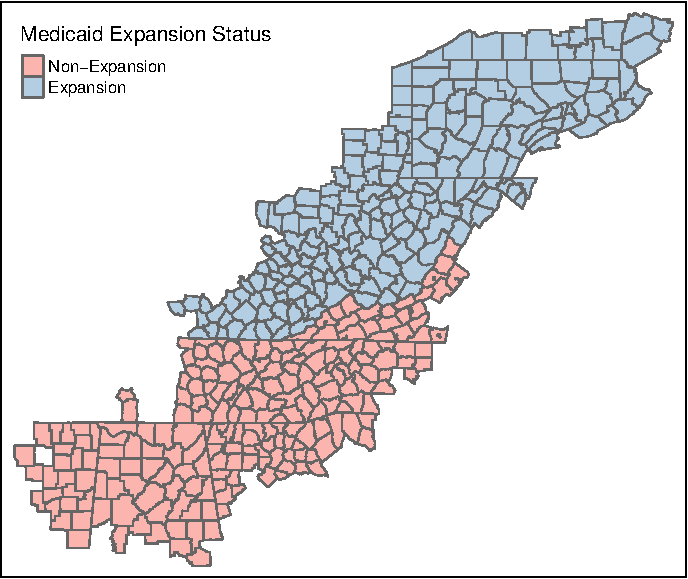
\includegraphics{figs/fig1.pdf}
\caption{Map of Medicaid Expansion Status Across Appalachian Counties}
\end{figure}

Clearly, at the state level there is a degree of ``North-South'' bias in
terms of which states elected to expand Medicaid. However, our empirical
strategy (as discussed in section 5) aims to minimize any associated
omitted variable bias with county-level fixed effects.

\hypertarget{variation-in-drug-overdose-death-rate}{%
\subsection{Variation in Drug Overdose Death
Rate}\label{variation-in-drug-overdose-death-rate}}

In Figure 2, we plot the weighted-average of county-level drug overdose
death rate over time (i.e., ``Years since Medicaid Expansion''),
separating counties in expansion states from counties in non-expansion
states.

\FloatBarrier

\begin{figure}
\centering
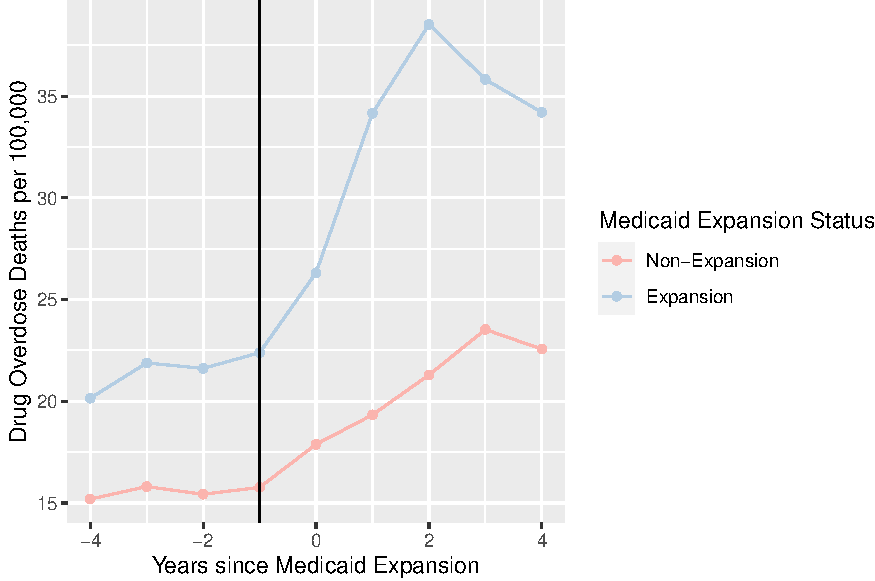
\includegraphics{figs/fig2.pdf}
\caption{Yearly County-Level Drug Overdose Death Rates by Medicaid
Expansion Status}
\end{figure}

\FloatBarrier

While drug overdose death rates are persistently higher in expansion
counties than in non-expansion counties, it appears that expansion
counties and non-expansion counties experience near-parallel trends
prior to Medicaid expansion. In the first few years following expansion,
however, we observe an \emph{steepening trend} of overdose death rates
in \emph{expansion counties} relative to \emph{non-expansion counties},
indicating that Medicaid expansion had a \emph{positive} effect on
overdose death rates, contradicting the direction of our hypothesized
causal effect.

Yet, we also observe that this steepening trend of overdose death rates
in expansion counties \emph{declines} following the first two years
after Medicaid expansion. Between years three and four after Medicaid
expansion, this trend reverses. Overall, this suggests that, to the
extent Medicaid expansion has increased overdose death rates in
expansion counties, this effect may be inconsistent over time. We
explore this possibility in our empirical strategy by employing an
``event study'' approach, which also allows us to more rigorously assess
the assumption of parallel trends.

\hypertarget{variation-in-key-continuous-variables}{%
\subsection{Variation in Key Continuous
Variables}\label{variation-in-key-continuous-variables}}

We also explore the balance across key continuous variables between
counties in expansion states and counties in non-expansion states, a
year prior to the time when Medicaid expansion occurs.

\begin{table}[H]

\caption{\label{tab:create diif in means}Difference-in-means between Expansion and Non-Expansion Counties, One Year Prior to Medicaid Expansion}
\centering
\begin{tabular}[t]{lrrrrrr}
\toprule
\multicolumn{1}{c}{ } & \multicolumn{2}{c}{Non-Expansion (N=213)} & \multicolumn{2}{c}{Expansion (N=210)} & \multicolumn{2}{c}{ } \\
\cmidrule(l{3pt}r{3pt}){2-3} \cmidrule(l{3pt}r{3pt}){4-5}
  & Mean & Std. Dev. & Mean & Std. Dev. & Diff. in Means & p\\
\midrule
Poverty Rate & 19.17 & 4.42 & 18.47 & 6.06 & -0.70 & 0.17\\
Median Age & 41.21 & 4.09 & 41.77 & 3.19 & 0.55 & 0.12\\
Male Share & 49.14 & 1.32 & 49.93 & 2.18 & 0.79 & <0.001\\
Black Share & 10.58 & 14.49 & 2.45 & 2.91 & -8.13 & <0.001\\
Hispanic Share & 4.00 & 4.10 & 1.55 & 1.60 & -2.45 & <0.001\\
White Share & 82.94 & 14.72 & 94.06 & 4.60 & 11.12 & <0.001\\
Asian Share & 0.69 & 1.09 & 0.53 & 0.91 & -0.16 & 0.10\\
\bottomrule
\multicolumn{7}{l}{\rule{0pt}{1em}Note: Observations are weighted by the population in each county.}\\
\end{tabular}
\end{table}

Table 1 shows difference-in-means between ``treatment'' (i.e., Medicaid
expansion) counties and ``control'' counties in the year of Medicaid
expansion. We observe statistically significant differences between
``treatment'' and ``control'' groups for male share of population and
racial composition (i.e., Black, White, and Hispanic share of
population). This suggests that these factors are unbalanced between the
two groups of Appalachian counties, which would lead to omitted variable
bias if they are not controlled for in our estimation specification.

\medspace

\hypertarget{empirical-strategy}{%
\section{Empirical Strategy}\label{empirical-strategy}}

The primary variation that we seek to exploit through our analysis is
the differential in state-level adoption of Medicaid expansion across
the Appalachian region, with policy variation at the state-level thus
filtering down to the county-level. We do this in two ways:

To establish a single average causal treatment effect estimate over the
five years after Medicaid was expanded, we first take a
difference-in-differences approach. This approach allows us to simply
establish evidence of a causal linkage between Medicaid expansion and
drug overdose deaths in Appalachia. We then go a step further by
exploring an event study approach, examining year-by-year treatment
effects relative to the year prior to Medicaid expansion. This second
approach allows us to demonstrate the robustness of our measured
treatment effect over time, and also provides a more granular lens to
critically assess the validity of the differences-in-differences result.

Finally, we look for heterogeneous treatment effects among ``high'' and
``low risk'' counties in both approaches.

\hypertarget{difference-in-differences}{%
\subsection{Difference-in-Differences}\label{difference-in-differences}}

To evaluate the effect of Medicaid expansion on drug overdose deaths in
Appalachian counties, we estimate the following
``differences-in-differences'' specification:

\[ODR_{it} = \beta Expansion_{it} + \textbf{X}_{it} \gamma + \nu_{i} + \tau_{t} + \varepsilon_{it}\]

where \(ODR_{it}\) is deaths attributed to drug overdose per 100,000
county residents for county \(i\) at time \(t\), \(Expansion_{it}\) is a
binary variable that indicates ``treatment'' status (i.e., enactment of
Medicaid expansion) for a county-year, \(\textbf{X}_{it}\) is a vector
of time varying controls (e.g., poverty rates, median age, male
population share, racial composition) for potential county-level
determinants of overdose death rates outside of our policy variation of
interest.

Additionally, we include an array of county fixed effects, \(\nu_{i}\),
that control for unobserved time-invariant factors that are specific to
individual counties. An example of one such factor would be if,
throughout the entire 2010-2019 period, a specific county had its own
drug treatment program that reduced drug overdose deaths compared to
other counties, all else equal. We further include \(\tau_{t}\), year
fixed effects, to control for unobserved county-invariant factors that
might have changed between each year included in our panel. Such factors
would include events such as periodic economic shocks that affect the
entire Appalachian region in certain years, which potentially could be
deterministic of the rate of overdose deaths. Finally,
\(\varepsilon_{it}\) is the idiosyncratic error term.

\hypertarget{event-study}{%
\subsection{Event Study}\label{event-study}}

In this approach, we apply a modified specification that isolates
treatments effects by year, before and after Medicaid expansion, which
corresponds to the following population regression function:

\[ODR_{it} =  1\{\text{Expansion}_i\} \left [ \sum_{y=-4}^{-2} \beta_y^{pre} 1\{t - t_i^* = y\} + \sum_{y=0}^{4} \beta_y^{post} 1\{t - t_i^* = y\}\right ] + \textbf{X}_{it} \gamma + \nu_{i} + \tau_{t} + \varepsilon_{it}\]
where \(1\{\text{Expansion}_i\}\) is a binary variable identifying
high-eligibility states, and \(t_i^*\) is the year Medicaid was expanded
in county \(i\). The \(1\{t - t_i^* = y\}\) terms are dummy variables
corresponding to an \emph{event year}, i.e., the year relative to the
expansion of Medicaid at time \(t_i^*\). The coefficients of interest
are \(\beta^{pre}_y\) and \(\beta^{post}_y\), which measure the
relationship between drug overdose death rates and expansion status in
each of the four years leading up to Medicaid expansion and five years
after. We omit the dummy for the year before Medicaid expansion
(\(y = -1\)), so that the estimates of \(\beta^{pre}_y\) and
\(\beta^{post}_y\) capture effects relative to just before Medicaid
expansion.

In particular, we measure \(\beta^{pre}_y\) parameters to capture the
relationship between expansion status and overdose death rates before
Medicaid was expanded, allowing us to establish the assumption of
parallel trends; statistically significant estimates during the
pre-treatment period would be inconsistent with the parallel trends
assumption, as this would indicate that expansion counties already
experienced a different trajectory of overdose death rates prior to the
expansion of Medicaid. The \(\beta^{post}_y\) parameters represent the
causal effect of Medicaid expansion for each event year (\(y\)) after
medicaid has been expanded.

Finally, we include the same vector of time-varying controls
(\(\textbf{X}_{it}\)), county fixed-effects (\(\nu_{i}\)), and year
fixed-effects (\(\tau_{t}\)), as specified in the
differences-in-differences approach.

\medspace

\hypertarget{findings}{%
\section{Findings}\label{findings}}

\hypertarget{difference-in-difference-results}{%
\subsection{Difference-in-Difference
Results}\label{difference-in-difference-results}}

We estimate difference-in-differences effects for all counties, ``high
risk,'' and ``low risk'' counties.

\begin{table}[!h]

\caption{\label{tab:estimate DID models}Effect of Medicaid Expansion on Drug Overdose Death Rates}
\centering
\resizebox{\linewidth}{!}{
\begin{tabular}[t]{l>{\centering\arraybackslash}p{2in}>{\centering\arraybackslash}p{2in}>{\centering\arraybackslash}p{2in}}
\toprule
  & All Counties & High Risk & Low Risk\\
\midrule
Medicaid Expansion & \num{5.6176}*** & \num{5.1436}*** & \num{4.5752}***\\
 & (\num{0.7056}) & (\num{0.7142}) & (\num{1.2315})\\
Poverty Rate (0-100) & \num{0.9121}*** & \num{0.4263}* & \num{0.7200}**\\
 & (\num{0.2106}) & (\num{0.2466}) & (\num{0.3263})\\
Median Age & \num{0.3399} & \num{-0.1889} & \num{0.4579}\\
 & (\num{0.2900}) & (\num{0.4612}) & (\num{0.4656})\\
Male Population Share (0-100) & \num{0.0001}** & \num{0.0000} & \num{0.0003}**\\
 & (\num{0.0000}) & (\num{0.0001}) & (\num{0.0001})\\
Black Population Share & \num{-0.0001}*** & \num{-0.0001} & \num{-0.0008}***\\
 & (\num{0.0000}) & (\num{0.0001}) & (\num{0.0003})\\
Hispanic Population Share & \num{-0.0000} & \num{0.0004}** & \num{-0.0008}\\
 & (\num{0.0001}) & (\num{0.0002}) & (\num{0.0007})\\
Asian Population Share & \num{0.0003} & \num{0.0005} & \num{0.0036}**\\
 & (\num{0.0003}) & (\num{0.0005}) & (\num{0.0016})\\
\midrule
N & \num{3807} & \num{1899} & \num{981}\\
R-squared & \num{0.760} & \num{0.801} & \num{0.866}\\
Adj. R-squared & \num{0.737} & \num{0.778} & \num{0.849}\\
County FEs & X & X & X\\
Year FEs & X & X & X\\
\bottomrule
\multicolumn{4}{l}{\rule{0pt}{1em}Robust standard errors clustered by county are shown in parentheses.
                      Observations are weighted by the population in each county.}\\
\multicolumn{4}{l}{\rule{0pt}{1em}* p $<$ 0.1, ** p $<$ 0.05, *** p $<$ 0.01}\\
\end{tabular}}
\end{table}

Table 2 displays difference-in-difference estimation results. We find
evidence that Medicaid expansion \emph{increased} the drug overdose
death rate by roughly 5.62 deaths per 100,000 across all Appalachian
counties in the post-expansion period, holding constant demographic
factors and county and time fixed effects. This effect is slightly
larger in ``high risk'' counties than it is in ``low risk'' counties,
although the difference is not substantial, and smaller in both
subgroups than it is across the entire sample. In all cases, this
estimate of causal effect is quite significant (\(\alpha < .01\)).

\hypertarget{event-study-results}{%
\subsection{Event Study Results}\label{event-study-results}}

For our event study approach, we plot \(\beta^{pre}_y\) and
\(\beta^{post}_y\) estimates for all counties, ``high risk,'' and ``low
risk'' counties in Figures 3-5. A complete table of event study approach
estimates, across all Appalachian counties, ``high risk,'' and ``low
risk'' counties, can be found in Appendix III, Table 5.

\begin{figure}
\centering
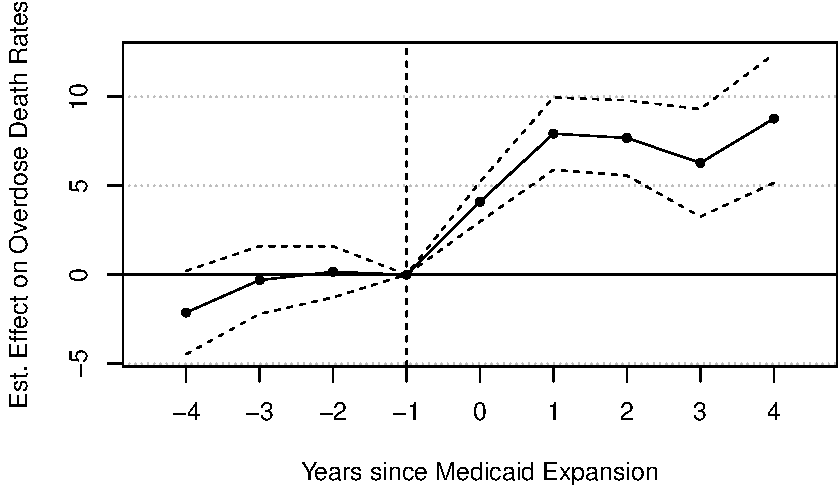
\includegraphics{figs/fig3.pdf}
\caption{Medicaid Expansion's Effect on Drug Overdose Death Rates in All
Appalachian Counties}
\end{figure}

Figure 3 displays the yearly estimated effect of Medicaid expansion on
drug overdose death rates across all counties Appalachia, before and
after expansion occurs. With regards to the pre-expansion
\(\beta^{pre}_y\) estimates, it appears that the assumption of parallel
trends mostly holds true, as the parameters are centered around zero and
are non statistically significant with the exception of \(y=-4\). The
\(\beta^{post}_y\) estimates show a \emph{positive} effect of Medicaid
expansion on drug overdose deaths that increases in the period
one-to-two years after Medicaid expansion, then stabilizes afterwards.
Together, \(\beta^{pre}_y\) and \(\beta^{post}_y\) estimates in the
event study approach largely conform to the results of the
difference-in-differences approach when analyzing all counties in
Appalachia.

\begin{figure}
\centering
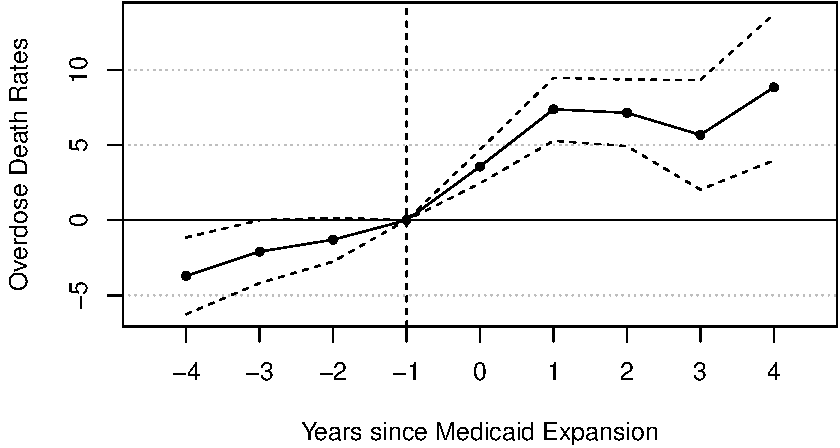
\includegraphics{figs/fig4.pdf}
\caption{Medicaid Expansion's Effect on Drug Overdose Death Rates in
High Risk Counties}
\end{figure}

\begin{figure}
\centering
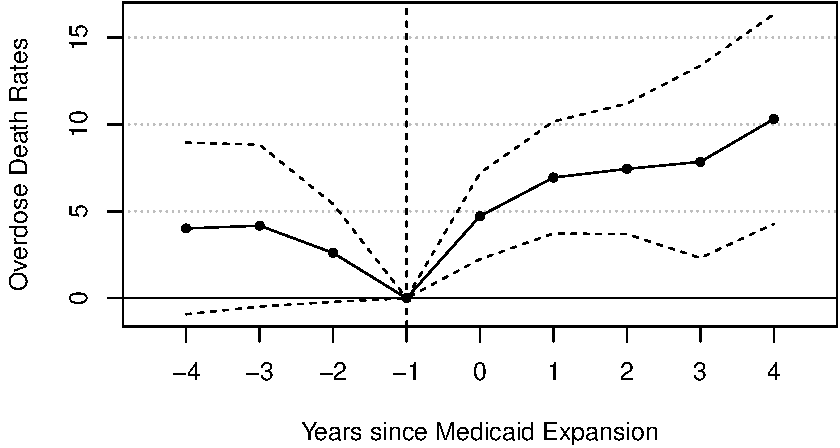
\includegraphics{figs/fig5.pdf}
\caption{Medicaid Expansion's Effect on Drug Overdose Death Rates in Low
Risk Counties}
\end{figure}

Figure 4 displays the yearly estimated effect of Medicaid expansion on
drug overdose death rates across ``high risk'' counties in Appalachia,
before and after expansion occurs. For the pre-expansion
\(\beta^{pre}_y\) estimates, it appears that the assumption of parallel
trends does not hold true. In the period four to one year prior to
Medicaid expansion, it appears that the time-trend in drug overdose
death rates is already diverging between expansion and non-expansion
counties, as the \(\beta^{pre}_y\) estimates are statistically
significant and are moving in an upwards direction over time. The
\(\beta^{post}_y\) estimates show a \emph{positive} effect of Medicaid
expansion on drug overdose deaths that increases in the period
one-to-two years after Medicaid expansion, afterwards causal effects
estimates stabilize but are increasingly noisy (i.e., widening 95\%
confidence intervals). Overall, the event study findings for ``high
risk'' counties cast doubt on the validity of difference-in-difference
results, as the assumption of parallel trends is shown to be dubious.

Figure 5 displays the yearly estimated effect of Medicaid expansion on
drug overdose death rates across ``low risk'' counties in Appalachia,
before and after expansion occurs. Based on the pre-expansion
\(\beta^{pre}_y\) estimates, the assumption of parallel trends also
appears to be fairly weak, as some of the \(\beta^{pre}_y\) estimates
are relatively statistically significant. Unlike the ``high risk''
county estimates, although the 95\% confidence interval is quite large,
the \(\beta^{pre}_y\) estimates actually suggest that the difference in
overdose death rates between expansion and non-expansion counties is
shrinking in ``low risk'' counties over the period up until one year
before expansion. Once again, \(\beta^{post}_y\) estimates show a
\emph{positive} effect of Medicaid expansion on drug overdose deaths
that increases in the period one-to-two years after Medicaid expansion,
only to stabilize afterwards. For ``low risk counties,'' in particular,
causal effect estimates are increasingly noisy after expansion (i.e.,
the 95\% confidence interval is very large and widening). The event
study findings for ``low risk'' counties cast some doubt on the validity
of difference-in-difference results because the assumption of parallel
trends is again not very strong, but the causal effects estimates are
fairly consistent with the possible exception of the final year
(\(y=4\)).

\medspace

\hypertarget{conclusion}{%
\section{Conclusion}\label{conclusion}}

\hypertarget{consistency-and-validity-of-findings}{%
\subsection{Consistency and Validity of
Findings}\label{consistency-and-validity-of-findings}}

Overall, we find that strong evidence \emph{against} our hypothesis that
Medicaid expansion would \emph{reduce} drug overdose death rates in
Appalachia. Causal effects estimates, both in the
difference-in-differences and event study approach, point in the
\emph{positive} direction when measured among all Appalachian counties,
``high risk'' counties, and ``low risk'' counties.

Instead, these results provide limited evidence to support the
counter-hypothesis that Medicaid expansion \emph{increased} drug
overdose death rates in Appalachia. When examining all counties in
Appalachia, the results of both difference-in-differences and event
study approaches suggest that a positive causal effect is likely.
However, the results from separate analysis of ``high risk'' and ``low
risk'' counties casts some doubt on this conclusion as well. First, the
assumption of parallel trends weakens when estimating causal effects for
these subsets, and also causal effects estimates for ``high risk''
counties are noisy. Second, the pattern of results for ``high'' and
``low risk'' counties does not conform with the mechanism proposed by
the counter hypothesis (i.e., Medicaid expansion increasing access to
prescription opioids), as this would have likely lead to a stronger
effect in ``low risk'' counties, but in fact our estimates are broadly
similar between the two groups.

If anything, the event study results do show evidence to support a claim
of lagged effects, as causal estimates are largest two-to-five years
after Medicaid expansion across all groups. This trajectory of effects
is theorized but not tested by
\href{https://onlinelibrary.wiley.com/doi/epdf/10.1111/add.14741}{Swartz
and Beltran (2019)}, who find that expansion increased the supply of
prescription opioids but did not affect overdose deaths.

We also cannot rule out the potential alternative hypothesis that
Medicaid expansion simply increased the ability of expansion counties to
collect data and attribute deaths to drug overdoses. This last
explanation would seem most consistent with the fact that the size of
our causal effects do not vary much by group, as we imagine this effect
would be rather agnostic to pre-expansion growth in overdose death
rates. To summarize, we find evidence against the original hypothesis
(i.e., Medicaid expansion reduced drug overdose deaths), but we also
cannot conclusively differentiate the evidence supporting the
counter-hypothesis from this possible alternative explanation.

Furthermore, there are a few key limitations that potentially challenge
the validity of this study. First, we are unable to control for
potential OVB due to county-year variation in number of substance use
disorder (SUD) treatment facilities, as this data was unavailable at the
county-level. However, it is unclear what the direction of this bias
would be. On one hand, SUD treatment facilities could be negatively
correlated with deaths from drug overdose due to the services that they
provide; on the other, it could also be the case that there are simply
more SUD treatment facilities in areas with high rates of drug overdose
deaths.

Lack of SUD treatment center data also impedes our ability to test the
mechanism behind our original hypothesis, as it is possible that the
effect of enhanced access to healthcare through Medicaid expansion on
drug overdose death rates would have been mediated by the presence of
SUD treatment centers. Second, we similarly lack data on the supply of
prescription opioids in Appalachian counties over this period, making it
difficult to assess the mechanism in the counter-hypothesis as well.
Finally, we believe that the focus of our sample on Appalachian counties
limits external validity, which potentially could explain the difference
between our results and prior research.

\hypertarget{policy-implications}{%
\subsection{Policy Implications}\label{policy-implications}}

With regards to policy, our results show that simply increasing access
the healthcare by itself is not a solution to the ongoing crisis of drug
overdose deaths in the United States, and possibly could be an
exacerbating factor. Our findings suggest, although weakly, that there
is a positive linkage between the healthcare system in Appalachia and
deaths from drug overdose. If this is indeed the case, then policymakers
ought to consider steps that decouple medical care (i.e., access to
doctors and prescription medication) from drug addiction. Interventions
suggested by experts include stronger limitations on amounts of opioids
prescribed, increasing access to rehabilitation treatment, and liability
placed on prescription drug companies
(\href{https://knowledge.wharton.upenn.edu/article/opioid-crisis-policy-solutions/}{University
of Pennslyvania, 2019}).

As for the Medicaid program in particular, it should be emphasized that,
even to the extent that these detrimental linkages exist, communities in
Appalachia are heavily reliant on the program to meet broader healthcare
needs and any potential reforms should be careful not to restrict access
to these critical services. Above all, it should be noted that the
evidence found in our study is quite ambiguous, and taken alone, does
not necessarily warrant decisive policy response.

\newpage

\hypertarget{appendices}{%
\section{Appendices}\label{appendices}}

\hypertarget{appendix-i-data-sources}{%
\subsection{Appendix I: Data Sources}\label{appendix-i-data-sources}}

We compile publicly-available data from the Appalachian Regional Council
(ARC), Kaiser Family Foundation (KFF), National Center for Health
Statistics (NCHS), and the US Census Bureau into a single county-year
panel data set.

\hypertarget{appalachian-counties}{%
\subsubsection{Appalachian Counties}\label{appalachian-counties}}

The Appalachian Regional Commission defines 423 counties in 13 states
(West Virginia, Alabama, Georgia, Kentucky, Maryland, Mississippi, New
York, North Carolina, Ohio, Pennsylvania, South Carolina, Tennessee, and
Virginia) as demarcating the Appalachian region. We adopt this
geographical definition in our research approach. More information
available at:
\url{https://www.arc.gov/appalachian-counties-served-by-arc/}.

\hypertarget{medicaid-expansion}{%
\subsubsection{Medicaid Expansion}\label{medicaid-expansion}}

According to the Kaiser Family Foundation, five states within Appalachia
(Kentucky, Maryland, New York, Ohio, and West Virginia) passed
legislation mandating the expansion of Medicaid as of January 1st, 2014.
Two additional states, Pennsylvania and Virginia, would later expand
Medicaid, with the former in 2015 and the latter in 2019. Six states
(Alabama, Georgia, Mississippi, North Carolina, South Carolina, and
Tennessee) have not expanded Medicaid to-date. Information on
state-level Medicaid expansion available at:
\url{https://www.kff.org/medicaid/issue-brief/status-of-state-medicaid-expansion-decisions-interactive-map/}.

\hypertarget{overdose-deaths}{%
\subsubsection{Overdose Deaths}\label{overdose-deaths}}

Our data on drug overdose deaths comes from estimates modeled by the
National Center for Health Statistics (NCHS), which are available at the
county-level for the period 2003-2020. Estimates are based on the
National Vital Statistics System multiple cause-of-death mortality
files. Populations used for computing death rates for 2011--2018 are
postcensal estimates based on the 2010 U.S. census. Rates for census
years are based on populations enumerated in the corresponding censuses.
Rates for noncensus years before 2010 are revised using updated
intercensal population estimates and may differ from rates previously
published.

Death rates for some states/counties and years may be low due to a high
number of unresolved pending cases or misclassification of ICD--10
(cause of death) codes for unintentional poisoning as R99, ``Other
ill-defined and unspecified causes of mortality.'' For example, this
issue is known to affect New Jersey in 2009 and West Virginia in 2005
and 2009 but also may affect other years and other states or counties.
Drug overdose death rates may be underestimated in those instances.
Source link:
\url{https://www.cdc.gov/nchs/data-visualization/drug-poisoning-mortality/}.

\hypertarget{county-level-demographics}{%
\subsubsection{County-Level
Demographics}\label{county-level-demographics}}

To control for time-variant, county-variant factors, we pull
county-level demographic data from the US Census Bureau's American
Community Survey (ACS), for years 2010-2019. Unfortunately, due to lack
of data for small-population counties, we are only able to use data from
the five-year edition of the ACS, likely obscuring time-variation among
the demographic measures. Specifically, we include factors such as
poverty rates, median age, male population share, and racial
composition.Data is downloaded from the US Census Bureau API using the R
package tidycensus.

\hypertarget{geographic-boundaries}{%
\subsubsection{Geographic Boundaries}\label{geographic-boundaries}}

In addition to county-level demographics, we pull county shapefiles from
the Census Bureau for mapping visuals:
\url{https://www.census.gov/geographies/mapping-files/time-series/geo/cartographic-boundary.html}

\newpage

\hypertarget{appendix-ii-defining-high-and-low-risk-counties}{%
\subsection{Appendix II: Defining ``High'' and ``Low Risk''
Counties}\label{appendix-ii-defining-high-and-low-risk-counties}}

To define ``high'' and ``low risk'' counties, we examine the trajectory
of drug overdose death rates in Appalachian counties prior to Medicaid
expansion. In particular, we calculate the annual growth rates of
overdose death rates in Appalachian counties in the pre-expansion period
(i.e., between one and four years prior to expansion).

\[Avg.~Pre~Expansion~Growth~Rate_{i} = 100 * \frac{1}{3} \sum_{t=-4}^{-2} \frac{ODR_{t+1} - ODR_t}{ODR_t}\]

Shown in Figure 6, growth of overdose death rates varies considerably
across Appalachian counties during this period, with some counties
experiencing a drastic reduction in overdose death rates, while others
see massive increases.

\begin{figure}
\centering
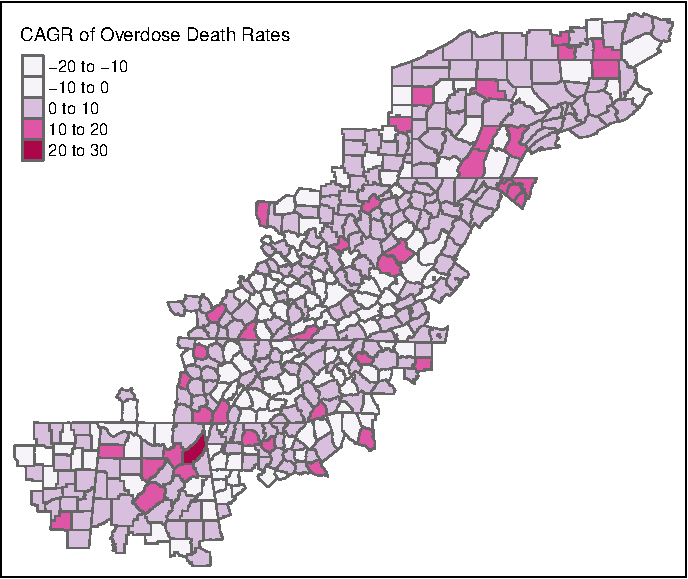
\includegraphics{figs/fig6.pdf}
\caption{Map of Pre-Expansion CAGR of Overdose Death Rates Across
Appalachian Counties}
\end{figure}

Over this period, annual average growth of overdose death rates ranged
from -16.31\% to 20.28\%, with a median of 3.68\%. We define ``high
risk'' counties as counties with average pre-expansion growth of drug
overdose death rates above the median, and define ``low risk'' counties
as counties with a pre-expansion growth of drug overdose death at or
below zero. Qualitatively, ``high risk'' counties can be thought of as
Appalachian counties that were already experiencing substantial
increases in drug overdose death rates prior to the expansion of
Medicaid. Conversely, ``low risk'' counties are counties where overdose
death rates were either stagnant or declining. Counties in between are
simply defined as ``moderate risk.''

From Table 3, it is evident that ``high risk'' counties are relatively
more concentrated among expansion counties, while ``low risk'' counties
are more concentrated among non-expansion counties. This lack of balance
likely impacts our estimates of causal effects among these subsets. In
our event study findings (see Appendix III), estimates for ``high'' and
``low'' risk counties are noisier than for all counties, so this
discrepancy could be a detriment to internal validity.

\begin{table}

\caption{\label{tab:twoway risk expansion}Two-Way Table of County Expansion and Risk Status}
\centering
\begin{tabular}[t]{l|c|c|c}
\hline
  & High & Low & Moderate\\
\hline
Non-Expansion & 93 & 63 & 57\\
\hline
Expansion & 118 & 46 & 46\\
\hline
\end{tabular}
\end{table}

We also explore demographic differences between ``high'' and ``low
risk'' counties, one year prior to Medicaid expansion.

\begin{table}[H]

\caption{\label{tab:diff_in_means_2}Difference-in-means between High and Low Risk Counties, One Year Prior to Medicaid Expansion}
\centering
\begin{tabular}[t]{lrrrrrr}
\toprule
\multicolumn{1}{c}{ } & \multicolumn{2}{c}{High (N=211)} & \multicolumn{2}{c}{Low (N=109)} & \multicolumn{2}{c}{ } \\
\cmidrule(l{3pt}r{3pt}){2-3} \cmidrule(l{3pt}r{3pt}){4-5}
  & Mean & Std. Dev. & Mean & Std. Dev. & Diff. in Means & p\\
\midrule
Poverty Rate & 18.22 & 5.20 & 19.82 & 5.33 & 1.60 & 0.01\\
Median Age & 41.61 & 3.61 & 40.84 & 3.38 & -0.77 & 0.06\\
Male Share & 49.38 & 1.32 & 49.56 & 2.37 & 0.18 & 0.47\\
Black Share & 6.35 & 11.43 & 6.33 & 8.67 & -0.02 & 0.98\\
Hispanic Share & 2.65 & 3.23 & 3.11 & 3.29 & 0.46 & 0.23\\
White Share & 88.76 & 12.00 & 88.08 & 11.40 & -0.68 & 0.62\\
Asian Share & 0.65 & 1.09 & 0.66 & 1.14 & 0.007 & 0.96\\
\bottomrule
\multicolumn{7}{l}{\rule{0pt}{1em}Note: Observations are weighted by the population in each county.}\\
\end{tabular}
\end{table}

From Table 4, we make the somewhat odd observation that ``high risk''
counties are poorer and older than ``low risk'' counties. This would
seem to run contrary to the established findings that poverty and youth
are factors that tend to \emph{increase} incidence of drug overdose
deaths. However, it could just be the case that these factors only
affect the \emph{level} of drug overdose death rates in a particular
county, but do not play a role in \emph{rates of growth}. In terms of
male population share and racial composition, however, there are no
statistically significant differences.

\newpage

\hypertarget{appendix-iii-event-study-estimates}{%
\subsection{Appendix III: Event Study
Estimates}\label{appendix-iii-event-study-estimates}}

\begin{table}[!h]

\caption{\label{tab:tabulate ES estimates}Effect of Medicaid Expansion on Drug Overdose Death Rates}
\centering
\begin{tabular}[t]{l>{\centering\arraybackslash}p{1.5in}>{\centering\arraybackslash}p{1.5in}>{\centering\arraybackslash}p{1.5in}}
\toprule
  & All Counties & High Risk & Low Risk\\
\midrule
(Year -4) * Expansion & \num{-2.1247}* & \num{-3.7093}*** & \num{4.0139}\\
 & (\num{1.1949}) & (\num{1.3042}) & (\num{2.5190})\\
(Year -3) * Expansion & \num{-0.3008} & \num{-2.0959}* & \num{4.1743}*\\
 & (\num{0.9706}) & (\num{1.0688}) & (\num{2.3752})\\
(Year -2) * Expansion & \num{0.1632} & \num{-1.3009}* & \num{2.6056}*\\
 & (\num{0.7323}) & (\num{0.7442}) & (\num{1.4357})\\
(Year 0) * Expansion & \num{4.0977}*** & \num{3.5690}*** & \num{4.7244}***\\
 & (\num{0.5692}) & (\num{0.5707}) & (\num{1.2648})\\
(Year 1) * Expansion & \num{7.9242}*** & \num{7.3800}*** & \num{6.9449}***\\
 & (\num{1.0366}) & (\num{1.0682}) & (\num{1.6436})\\
(Year 2) * Expansion & \num{7.6838}*** & \num{7.1457}*** & \num{7.4423}***\\
 & (\num{1.0774}) & (\num{1.1325}) & (\num{1.9165})\\
(Year 3) * Expansion & \num{6.2820}*** & \num{5.6779}*** & \num{7.8475}***\\
 & (\num{1.5417}) & (\num{1.8601}) & (\num{2.8231})\\
(Year 4) * Expansion & \num{8.7733}*** & \num{8.8411}*** & \num{10.3101}***\\
 & (\num{1.8434}) & (\num{2.4835}) & (\num{3.0762})\\
\midrule
N & \num{3807} & \num{1899} & \num{981}\\
R-squared & \num{0.771} & \num{0.817} & \num{0.872}\\
Adj. R-squared & \num{0.749} & \num{0.795} & \num{0.854}\\
County FEs & X & X & X\\
Year FEs & X & X & X\\
\bottomrule
\multicolumn{4}{l}{\rule{0pt}{1em}Control covariates include county-level poverty rate, median age, male pop. share, Black pop. share,}\\
\multicolumn{4}{l}{\rule{0pt}{1em}White pop. share, Hispanic pop. share, and Asian pop. share.}\\
\multicolumn{4}{l}{\rule{0pt}{1em}Robust standard errors clustered by county are shown in parentheses.}\\
\multicolumn{4}{l}{\rule{0pt}{1em}Observations are weighted by the population in each county.}\\
\multicolumn{4}{l}{\rule{0pt}{1em}* p $<$ 0.1, ** p $<$ 0.05, *** p $<$ 0.01}\\
\end{tabular}
\end{table}

\end{document}
